\documentclass[tikz,border=4pt]{standalone}
\usepackage{tikz}
\usepackage{amsmath}
\usetikzlibrary{calc,arrows.meta,positioning,shapes.geometric,patterns}

\begin{document}
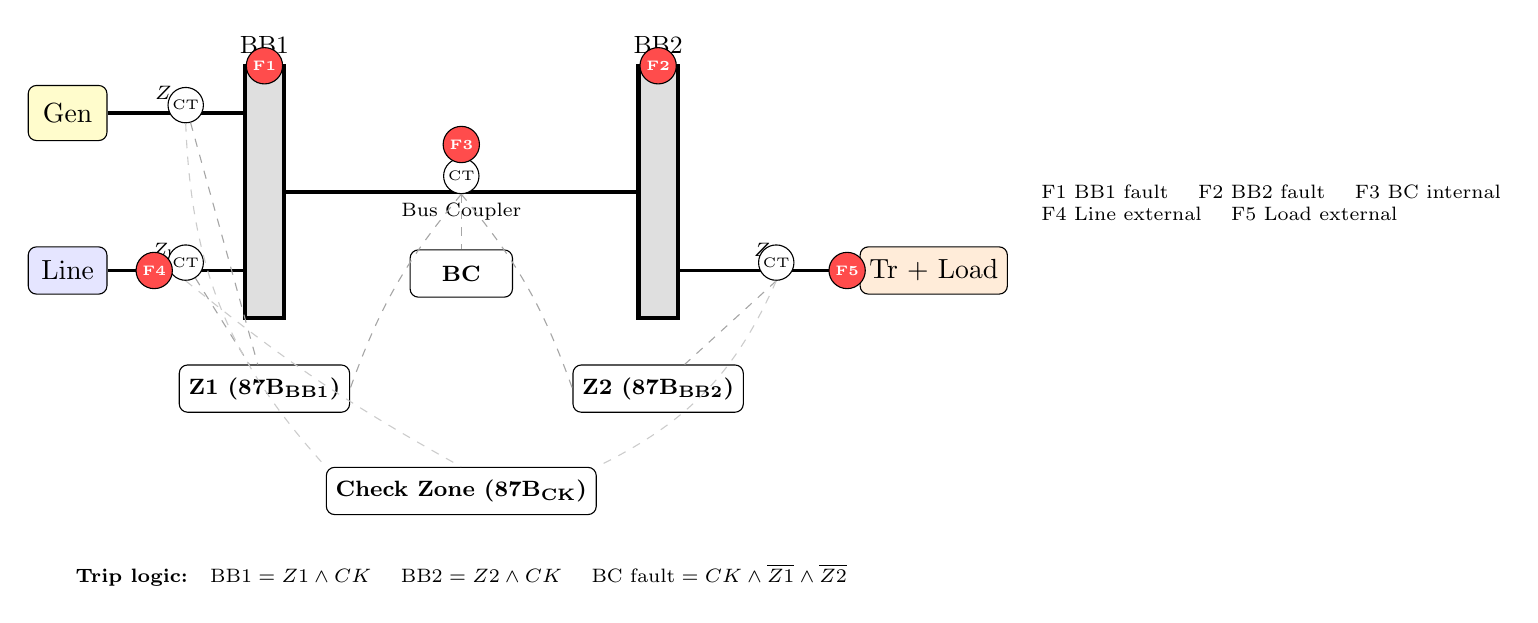
\begin{tikzpicture}[
    bus/.style={draw,fill=gray!25,minimum width=0.5cm,minimum height=3.2cm,
                line width=1.5pt,inner sep=0pt},
    relay/.style={draw,fill=white,rounded corners=3pt,
                  font=\footnotesize\bfseries,
                  minimum width=1.3cm,minimum height=0.6cm},
    zone/.style={draw,dashed,rounded corners=5pt,line width=0.9pt},
    ct/.style={draw,circle,fill=white,inner sep=1pt,font=\tiny,
               minimum size=0.3cm},
    arr/.style={-{Latex[length=2.5mm]},line width=0.8pt},
    fault/.style={draw,fill=red!70,circle,inner sep=1.5pt,
                  font=\tiny\bfseries,text=white},
    ann/.style={font=\scriptsize},
]

% ---- Buses ---------------------------------------------------------------
\node[bus,label={[font=\small]above:BB1}] (bb1) at (3,0)  {};
\node[bus,label={[font=\small]above:BB2}] (bb2) at (8,0)  {};

% ---- Generator -----------------------------------------------------------
\node[draw,fill=yellow!20,rounded corners=3pt,minimum width=1cm,
      minimum height=0.7cm] (gen) at (0.5,1.0) {Gen};
\draw[line width=1.2pt] (gen.east) -- (bb1.west|-gen.east)
    node[midway,above,ann]{$Z_{\rm src}$};

% ---- Gen CT
\node[ct] (ct_gen) at (2.0,1.1) {\tiny CT};

% ---- Line feeder ---------------------------------------------------------
\node[draw,fill=blue!10,rounded corners=3pt,minimum width=1cm,
      minimum height=0.6cm] (line) at (0.5,-1.0) {Line};
\draw[line width=1.2pt] (line.east) -- (bb1.west|-line.east)
    node[midway,above,ann]{$Z_{\rm line}$};
\node[ct] (ct_line) at (2.0,-0.9) {\tiny CT};

% ---- Bus Coupler ---------------------------------------------------------
\draw[line width=1.5pt] (bb1.east|-{(0,0)}) -- (bb2.west|-{(0,0)})
    node[midway,above,ann]{$Z_{\rm bc}$}
    node[midway,below,ann]{Bus Coupler};
\node[ct] (ct_bc) at (5.5,0.2) {\tiny CT};
% BC relay
\node[relay,below=0.7cm of ct_bc] (rBC) {BC};
\draw[dashed,gray!70] (ct_bc) -- (rBC);

% ---- Transformer feeder --------------------------------------------------
\node[draw,fill=orange!15,rounded corners=3pt,minimum width=1cm,
      minimum height=0.6cm] (tr) at (11.5,-1.0) {Tr + Load};
\draw[line width=1.2pt] (bb2.east|-tr.west) -- (tr.west)
    node[midway,above,ann]{$Z_{\rm tr}$};
\node[ct] (ct_tr) at (9.5,-0.9) {\tiny CT};

% ---- Zone 1 relay --------------------------------------------------------
\node[relay] (rZ1) at (3,-2.5) {Z1 (87B\textsubscript{BB1})};
\draw[dashed,gray!70] (ct_gen)  -- (rZ1);
\draw[dashed,gray!70] (ct_line) -- (rZ1);
\draw[dashed,gray!70] (ct_bc.south) to[bend right=10] (rZ1.east);

% ---- Zone 2 relay --------------------------------------------------------
\node[relay] (rZ2) at (8,-2.5) {Z2 (87B\textsubscript{BB2})};
\draw[dashed,gray!70] (ct_tr.south)  -- (rZ2);
\draw[dashed,gray!70] (ct_bc.south) to[bend left=10] (rZ2.west);

% ---- Check zone relay ----------------------------------------------------
\node[relay,minimum width=2.8cm] (rCK) at (5.5,-3.8) {Check Zone (87B\textsubscript{CK})};
\draw[dashed,gray!40] (ct_gen.south)  to[bend right=20] (rCK.north west);
\draw[dashed,gray!40] (ct_line.south) to[bend right=5]  (rCK.north);
\draw[dashed,gray!40] (ct_tr.south)   to[bend left=20]  (rCK.north east);

% ---- Fault markers -------------------------------------------------------
\node[fault] at (3, 1.6) {F1};
\node[fault] at (8, 1.6) {F2};
\node[fault] at (5.5,0.6) {F3};
\node[fault] at (1.6,-1.0) {F4};
\node[fault] at (10.4,-1.0) {F5};

% ---- Trip logic annotation -----------------------------------------------
\node[font=\scriptsize,align=left,below=0.5cm of rCK.south]
    {\textbf{Trip logic:}\quad
     $\text{BB1}=Z1\wedge CK$ \quad
     $\text{BB2}=Z2\wedge CK$ \quad
     $\text{BC fault}=CK\wedge\overline{Z1}\wedge\overline{Z2}$};

% ---- Legend --------------------------------------------------------------
\node[font=\scriptsize,above right=0.2cm and 0.3cm of tr.north east,align=left]
    {F1 BB1 fault \quad F2 BB2 fault \quad F3 BC internal\\
     F4 Line external \quad F5 Load external};

\end{tikzpicture}
\end{document}
